% !TeX program = XeLaTeX
% !TeX root = main.tex
% Edit by:刘力手 and 杨彦坡
\chapter{多元数量值函数积分学}\label{cha:5}
%chapter函数定义标题,{}内部写上文字,
%至于\label{cha:5}不是很清楚什么意思
\section{二重积分}%%5.1节
\begin{xiti}
	\item 设$D$为中心在原点,半径为$r$的圆域,求$\lim _{r \rightarrow 0} \frac{1}{\pi r^{2}} \iint_{D} \mathrm{e}^{x^{2}-y^{2}} \cos (x+y) \mathrm{d} x \mathrm{d} y$
	\begin{solution}
		由二重积分的积分中值定理知存在$(\xi, \eta) \in D$,使得
		\[\iint_{D} \mathrm{e}^{x^{2}-y^{2}} \cos (x+y) \mathrm{d} x \mathrm{d} y=\pi r^{2} \mathrm{e}^{\xi^{2}-\eta^{2}} \cos (\xi+\eta)\]由于当$r \rightarrow 0$,故$(\xi, \eta) \rightarrow(0,0)$,于是有\[\lim _{r \rightarrow 0} \frac{1}{\pi r^{2}} \iint_{D} \mathrm{e}^{x^{2}-y^{2}} \cos (x+y) \mathrm{d} x \mathrm{d} y=\lim _{r \rightarrow 0} \mathrm{e}^{\xi^{2}-\eta^{2}} \cos (\xi+\eta)=1\]
		\begin{note}
			二重积分的积分中值定理:设$f(x,y)$在区域$D$上连续,则存在$(\xi, \eta) \in D$,使得$\iint_{D} f(x,y) \mathrm{d} x \mathrm{d} y= f(\xi,\eta) \cdot \iint_{D} \mathrm{d} x \mathrm{d} y= f(\xi,\eta) \cdot S_{D}$
		\end{note}
	\end{solution}
	\item 求$\iint_{D} x y\left[1+x^{2}+y^{2}\right] \mathrm{d} \sigma$,其中$D=\left\{(x, y) | x^{2}+y^{2} \leqslant \sqrt{2}, x \geqslant 0, y \geqslant 0\right\}$,其中$[\cdot]$为取整函数.
	\begin{solution}
		原式$=\int_{0}^{\frac{\pi}{2}} \mathrm{d} \theta \int_{0}^{\sqrt[4]{2}} r \cos \theta \cdot r \sin \theta\left[1+r^{2}\right] r \mathrm{d} r=\int_{0}^{\frac{\pi}{2}} \sin \theta \cos \theta \mathrm{d} \theta \int_{0}^{\sqrt[4]{2}} r \cdot r\left[1+r^{2}\right] r \mathrm{d} r$
		
		$=\left.\frac{(\sin \theta)^{2}}{2}\right|_{0} ^{\frac{\pi}{2}} \cdot \frac{1}{2} \int_{0}^{\sqrt[4]{2}} r^{2}\left[1+r^{2}\right]d\left(r^{2}\right) \xlongequal{{r^2} + 1 = u} \frac{1}{2} \cdot \frac{1}{2} \int_{1}^{1+\sqrt{2}}(u-1)[u] \mathrm{d} u $
				
		$=\frac{1}{4}\left\{\int_{1}^{2}(u-1) \mathrm{d} u+\int_{2}^{1+\sqrt{2}} 2(u-1) \mathrm{d} u\right\}=\frac{1}{4}\left(\int_{0}^{1} t \mathrm{d} t+\int_{1}^{\sqrt{2}} 2 t \mathrm{d} t\right)=\frac{1}{4}\left(\frac{1}{2}+2-1\right)=\frac{3}{8}$
	\end{solution}
	\item 计算$\int_{0}^{1} \mathrm{d} x \int_{\sqrt{x}}^{x} \sin \frac{\pi x}{2 y} \mathrm{d} y+\int_{2}^{4} \mathrm{d} x \int_{\sqrt{x}}^{2} \sin \frac{\pi x}{2 y} \mathrm{d} y$.
	\begin{note}
		本题有误,应改为$\int_{1}^{2} \mathrm{d} x \int_{\sqrt{x}}^{x} \sin \frac{\pi x}{2 y} \mathrm{d} y+\int_{2}^{4} \mathrm{d} x \int_{\sqrt{x}}^{2} \sin \frac{\pi x}{2 y} \mathrm{d} y$	
	\end{note}
	\begin{solution}
		积分区域如下图所示:(紫色区域表示的是前面一部分的积分区域,褐色部分表示的是后面一部分的积分区域,下图为geogebra软件制作,由刘力手和本本蛋蛋提供,在此做出感谢)
		
		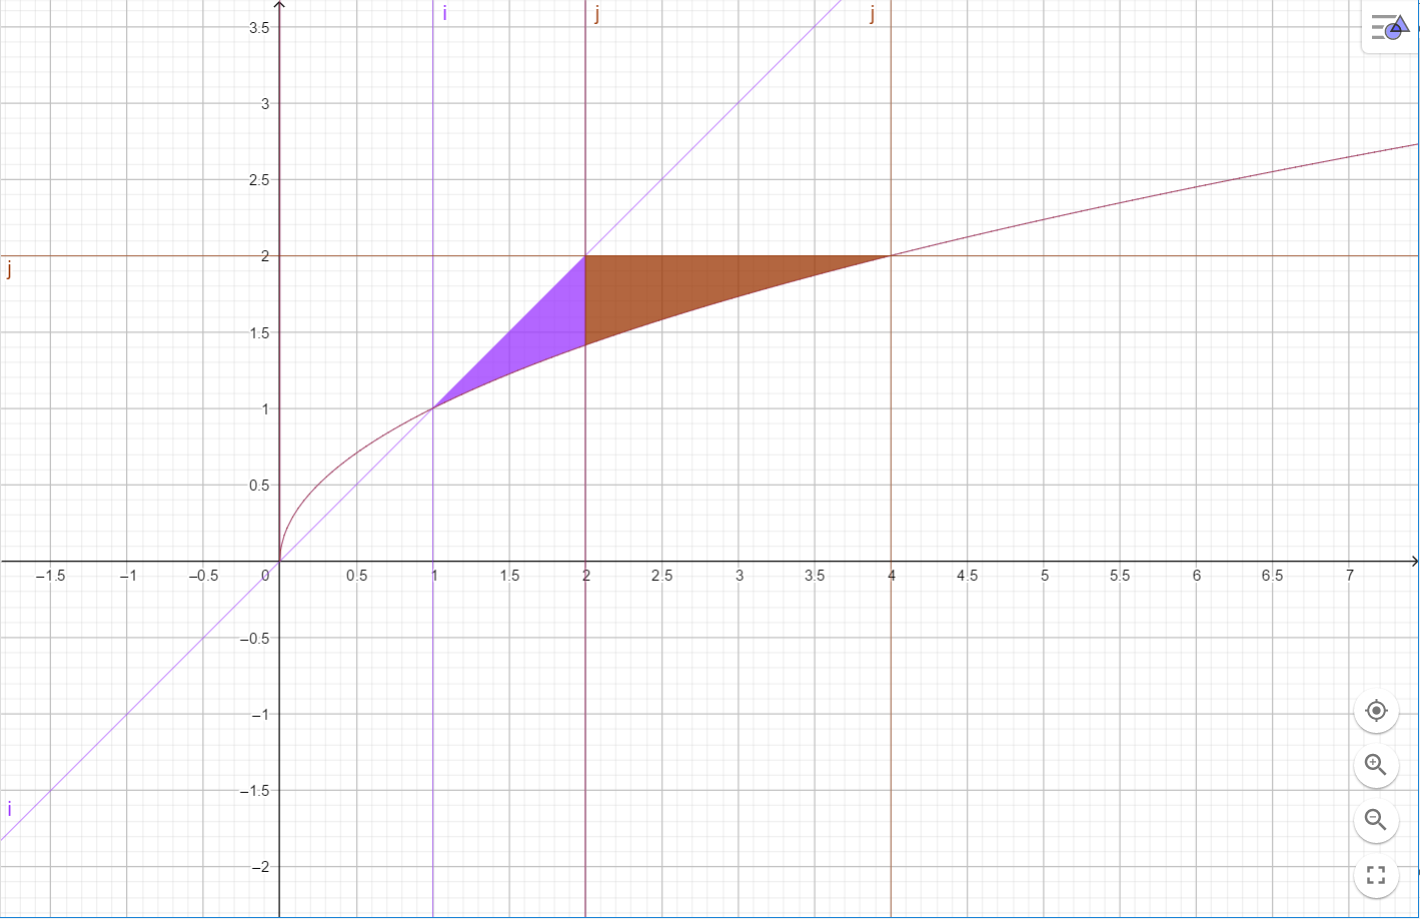
\includegraphics[width=0.80\textwidth]{Problem_3.png}
	
		则原式$=\int_{1}^{2} \mathrm{d} y \int_{y}^{y^{2}} \sin \frac{\pi x}{2 y} \mathrm{d} x=\int_{1}^{2} \mathrm{d} y\left(\frac{2}{\pi} y \int_{\frac{\pi}{2}}^{\frac{\pi}{2} y} \sin u \mathrm{d} u\right)=-\int_{1}^{2}\left(\frac{2}{\pi} y \cos \frac{\pi}{2} y\right) \mathrm{d} y$
		
		$\xlongequal{\frac{\pi}{2}y = t }-\left(\frac{2}{\pi}\right)^{3} \int_{\frac{\pi}{2}}^{\pi} t \cos t \mathrm{d} t=-\frac{8}{\pi^{3}}\left.(t \sin t+\cos t)\right|_{\frac{\pi}{2}} ^{\pi}=\frac{8}{\pi^{3}}\left(1+\frac{\pi}{2}\right)=\frac{4(2+\pi)}{\pi^{3}}$
		
		\begin{note}
			本题考察的是交换积分次序(前提是得正确画出区域)
		\end{note}
	\end{solution}
	\item 计算二重积分$\iint_{D} \mathrm{e}^{\max \left\{x^{2}, y^{2}\right\rangle} \mathrm{d} x \mathrm{d} y$,其中$D=\{(x, y)|0 \leqslant x \leqslant 1, \quad 0 \leqslant y \leqslant 1|\}$.
	%解答题
	\begin{solution}
		记$D_{1}=\{(x, y) | 0 \leq x \leq 1,0 \leq y \leq x\}$,$D_{2}=\{(x, y) | 0 \leq x \leq 1, x \leq y \leq 1\}$
		
		由于区域$D_{1}$和区域$D_{2}$关于$y=x$对称
		
		故$\iint_{D_{1}} \mathrm{e}^{\max \left\{x^{2}, y^{2}\right\}} \mathrm{d} x \mathrm{d} y=\iint_{D_{2}} \mathrm{e}^{\max \left\{y^{2}, x^{2}\right\}} \mathrm{d} x \mathrm{d} y$
		
		故原式$=2 \iint_{D_{1}} \mathrm{e}^{\max \left\{x^{2}, y^{2}\right\}} \mathrm{d} x \mathrm{d} y=2 \iint_{D_{1}} \mathrm{e}^{x^{2}} \mathrm{d} x \mathrm{d} y=2 \int_{0}^{1} \mathrm{d} x \int_{0}^{x} \mathrm{e}^{x^{2}} \mathrm{d} y=2 \int_{0}^{1} x \mathrm{e}^{x^{2}} \mathrm{d} x=\mathrm{e}-1$
		
		\begin{note}
			
			1.如果积分区域$D$关于$x,y$具有轮换对称性,也就是$D$当中如果交换$x$和$y$的位置的话,区域表示结果一模一样,且假定区域$D_{1}$为区域$D$的$y=x$的一侧,那么我们就可以得到$\iint_{D} f(x,y) \mathrm{d} x \mathrm{d} y= \iint_{D} f(y,x) \mathrm{d} x \mathrm{d} y = 2\iint_{D_{1}} f(x,y) \mathrm{d} x \mathrm{d} y$
			
			2.注意:$\int e^{x^{2}} \mathrm{d} x$无初等函数(也就是俗称的“不可积”)
		\end{note}
	\end{solution}
	%解答题的解答
	\item 设函数$f(x)$在$[0,1]$上连续,并设$\int_{0}^{1} f(x) \mathrm{d} x=A$,求$I=\int_{0}^{1} \mathrm{d} x \int_{x}^{1} f(x) f(y) \mathrm{d} y$.
	%解答题
	\begin{solution}
		法1:$I=\int_{0}^{1} \mathrm{d} x \int_{x}^{1} f(x) f(y) \mathrm{d} y=\int_{0}^{1}\left[f(x) \int_{x}^{1} f(y) \mathrm{d} y\right] \mathrm{d} x=-\int_{0}^{1}\left[\int_{x}^{1} f(y) \mathrm{d} y\right] \mathrm{d}\left[\int_{x}^{1} f(y) \mathrm{d} y\right]$
		$=-\frac{1}{2}\left.\left[\int_{x}^{1} f(y) \mathrm{d} y\right]^{2}\right|_{0} ^{1}=\frac{1}{2}\left[\int_{0}^{1} f(y) \mathrm{d} y\right]^{2}=\frac{1}{2}\left[\int_{0}^{1} f(x) \mathrm{d} x\right]^{2}=\frac{A^{2}}{2}$
		
		法2:$I=\int_{0}^{1} \mathrm{d} x \int_{x}^{1} f(x) f(y) \mathrm{d} y=\int_{0}^{1} \mathrm{d} y \int_{0}^{y} f(x) f(y) \mathrm{d} x=\int_{0}^{1}\left[f(y) \int_{0}^{y} f(x) \mathrm{d} x\right] \mathrm{d} y$
		$=\int_{0}^{1}\left[\int_{0}^{y} f(x) \mathrm{d} x\right] \mathrm{d}\left[\int_{0}^{y} f(x) \mathrm{d} x\right]=\frac{1}{2}\left.\left[\int_{0}^{y} f(x) \mathrm{d} x\right]^{2}\right|_{0} ^{1}=\frac{1}{2}\left[\int_{0}^{1} f(x) \mathrm{d} x\right]^{2}=\frac{A^{2}}{2}$
		
		法3:$I=\int_{0}^{1} \mathrm{d} x \int_{x}^{1} f(x) f(y) \mathrm{d} y=\int_{0}^{1} \mathrm{d} y \int_{0}^{y} f(x) f(y) \mathrm{d} x=\int_{0}^{1} \mathrm{d} y \int_{y}^{1} f(y) f(x) \mathrm{d} x$
		\\$=\frac{1}{2} \int_{0}^{1} \mathrm{d} y \int_{0}^{1} f(x) f(y) \mathrm{d} x=\frac{1}{2} \int_{0}^{1} f(y) \mathrm{d} y \cdot \int_{0}^{1} f(x) \mathrm{d} x=\frac{1}{2}\left[\int_{0}^{1} f(x) \mathrm{d} x\right]^{2}=\frac{A^{2}}{2}$
	\end{solution}
	%解答题的解答
	\item 计算积分$\iint_{D}(x+y) \mathrm{d} x \mathrm{d}y$,其中$D=\left\{(x, y) | x^{2}+y^{2} \leqslant 2 x+2 y\right\}$.
	%解答题
	\begin{solution}
		法1:区域$D=\left\{(x, y) |(x-1)^{2}+(y-1)^{2} \leq 2\right\}$
		
		故令$x-1=u, y=1=v$,则$\mathrm{d} x \mathrm{d} y=\mathrm{d} u \mathrm{d} v$,区域$D_{1}=\left\{(u, v) | u^{2}+v^{2} \leq 2\right\}$
		
		故原式$=\iint_{D_{1}}[(u+1)+(v+1)] \mathrm{d} u \mathrm{d} v=\iint_{D_{1}} 2 \mathrm{d} u \mathrm{d} v=2 \cdot 2 \pi=4 \pi$
		
		法2:原式$=\int_{-\frac{\pi}{4}}^{3 \pi} \mathrm{d} \theta \int_{0}^{2 \cos \theta+2 \sin \theta}(r \cos \theta+r \sin \theta) r \mathrm{d} r=\int_{-\frac{\pi}{4}}^{3 \pi} \frac{(2 \cos \theta+2 \sin \theta)^{3}(\cos \theta+\sin \theta)}{3} \mathrm{d} \theta$
		$=\frac{8}{3} \int_{-\frac{\pi}{4}}^{3 \pi}(\cos \theta+\sin \theta)^{4} \mathrm{d} \theta=\frac{8}{3} \int_{-\frac{\pi}{4}}^{\frac{3 \pi}{4}}\left[\sqrt{2} \sin \left(\theta+\frac{\pi}{4}\right)\right]^{4} \mathrm{d} \theta=\frac{32}{3} \int_{0}^{\pi} \sin ^{4} \theta \mathrm{d} \theta=\frac{32}{3} \cdot 2 \cdot \frac{3}{4} \cdot \frac{1}{2} \cdot \frac{\pi}{2}=4 \pi$
		
		\begin{conclusion}
			华里士公式:$\int_{0}^{\frac{\pi}{2}} \sin^{n} x \mathrm{d} x = \int_{0}^{\frac{\pi}{2}} \cos^{n} x \mathrm{d} x = \left\{\begin{array}{l}{\frac{n-1}{n} \cdot \frac{n-3}{n-2} \cdot \cdot \cdot \frac{2}{3} , n  \text{为奇数}} \\\\ {\frac{n-1}{n} \cdot \frac{n-3}{n-2} \cdot \cdot \cdot \frac{1}{2} \cdot \frac{\pi}{2} , n \text{为偶数}}\end{array}\right.$
		\end{conclusion}
	%%text{文字$数学公式$}
	\end{solution}
	%解答题的解答
	\item 计算$\int_{0}^{a} \mathrm{d} x \int_{-x}^{-a+\sqrt{a^{2}-x^{2}}} \frac{1}{\sqrt{x^{2}+y^{2}}} \frac{1}{\sqrt{4 a^{2}-x^{2}-y^{2}}} \mathrm{d} y (a>0)$
	%解答题
	\begin{solution}
		原式$=\int_{-\frac{\pi}{4}}^{0} \mathrm{d} \theta \int_{0}^{-2 a \sin \theta} \frac{1}{r} \frac{r}{\sqrt{4 a^{2}-r^{2}}} \mathrm{d} r=\int_{-\frac{\pi}{4}}^{0}\left.\left(\arcsin \frac{r}{2 a}\right)\right|_{0} ^{-2 a \sin \theta} \mathrm{d} \theta=\int_{-\frac{\pi}{4}}^{0}(-\theta) \mathrm{d} \theta=\frac{\pi^{2}}{32}$
	\end{solution}
	%解答题的解答
	\item 计算$\iint_{D} |\sin (x-y) | \mathrm{d} \sigma, D : 0 \leqslant x \leqslant y \leqslant 2 \pi$
	%解答题
	\begin{solution}
		法1:记$D_{1} :\{(x, y) | 0 \leq x \leq y \leq 2 \pi, 0 \leq y-x \leq \pi\}$,$D_{2} :\{(x, y) | 0 \leq x \leq y \leq 2 \pi, \pi<y-x \leq 2 \pi\}$
		
		故原式$=\iint_{D_{1}}|\sin (x-y)| \mathrm{d} \sigma+\iint_{D_{2}}|\sin (x-y)| \mathrm{d} \sigma=\iint_{D_{1}} \sin (y-x) \mathrm{d} \sigma-\iint_{D_{2}} \sin (y-x) \mathrm{d} \sigma$
		$=\iint_{D} \sin (y-x) \mathrm{d} \sigma-2 \iint_{D_{2}} \sin (y-x) \mathrm{d} \sigma=\int_{0}^{2 \pi} \mathrm{d} y \int_{0}^{y} \sin (y-x) \mathrm{d} x-2 \int_{\pi}^{2 \pi} \mathrm{d} y \int_{0}^{y-\pi} \sin (y-x) \mathrm{d} x$
		$=\int_{0}^{2 \pi} \mathrm{d} y \int_{0}^{y} \sin x \mathrm{d} x+2 \int_{\pi}^{2 \pi} \mathrm{d} y \int_{\pi}^{y} \sin t \mathrm{d} t=\int_{0}^{2 \pi}(1-\cos y) \mathrm{d} y+2 \int_{\pi}^{2 \pi}(1-\cos y) \mathrm{d} y$
		$=2 \pi+2 \int_{\pi}^{2 \pi}(1-\cos y) \mathrm{d} y=4 \pi-2 \int_{\pi}^{2 \pi} \cos y \mathrm{d} y=4 \pi$
		
		法2:原式$=\int_{0}^{2 \pi} \mathrm{d} y \int_{0}^{y}|\sin (x-y)| \mathrm{d} x=\int_{0}^{2 \pi} \mathrm{d} y \int_{0}^{y}|\sin x| \mathrm{d} x=\left.\left(y \int_{0}^{y}|\sin x| \mathrm{d} x\right)\right|_{0} ^{2 \pi}-\int_{0}^{2 \pi} y|\sin y| \mathrm{d} y$
		$=2 \pi \int_{0}^{2 \pi}|\sin x| \mathrm{d} x-\pi \int_{0}^{2 \pi}|\sin y| \mathrm{d} y=\pi \int_{0}^{2 \pi}|\sin y| \mathrm{d} y=\pi \cdot 2 \cdot 2=4 \pi$
		
		\begin{note}
		$\int_{0}^{2 \pi} y|\sin y| \mathrm{d} y=\pi \int_{0}^{2 \pi}|\sin y| \mathrm{d} y$的理由如下:
		
		$\int_{0}^{2 \pi} y|\sin y| \mathrm{d} y=\int_{0}^{2 \pi-y=t}(2 \pi-t)|\sin t| \mathrm{d} t=\int_{0}^{2 \pi} 2 \pi|\sin t| \mathrm{d} t-\int_{0}^{2 \pi} t \sin t | \mathrm{d} t$
		
		故$\int_{0}^{2 \pi} y|\sin y| \mathrm{d} y=\pi \int_{0}^{2 \pi}|\sin y| \mathrm{d} y$
		\end{note}
	\end{solution}
	%解答题的解答
	\item 计算积分$\iint_{D}(x+y) \mathrm{d} x \mathrm{d}y$,其中$D=\left\{(x, y) | y^{2} \leqslant x+2, x^{2} \leqslant y+2\right\}$.
	%解答题
	\begin{solution}
		记$D_{1}=\left\{(x, y) | y^{2} \leqslant x+2, x^{2} \leqslant y+2, y \leqslant x \right\}$,$D_{1}$的边界为$L$
		
		其中$L$是由$L_{1},L_{2},L_{3}$所围成的,这三条线分别为
		
		$L_{1}:y=x$,$x$从$2$到$-1$;
		
		$L_{2}:y^{2}=x+2$,$y$从$-1$到$-\frac{\sqrt{5}+1}{2}$;
		
		$L_{3}:x^{2}=y+2$,$x$从$\frac{\sqrt{5}-1}{2}$到$2$.
		
		则原式$=2 \iint_{D_{1}}(x+y) \mathrm{d} x \mathrm{d} y= \int_{L} (x-y^{2}) \mathrm{d} x + (x^{2}-y) \mathrm{d} ys$
		
		$=\int_{L_{2}}\left(x-y^{2}\right) \mathrm{d}x+\left(x^{2}-y\right) \mathrm{d}y+\int_{L_{3}}\left(x-y^{2}\right) \mathrm{d}x+\left(x^{2}-y\right) \mathrm{d}y $
		
		$=\int_{-1}^{-\frac{\sqrt{5}+1}{2}}\left[(-2) \cdot 2 y+\left(y^{2}-2\right)^{2}-y\right] \mathrm{d}y+\int_{\frac{\sqrt{5}-1}{2}}^{2}\left[x-\left(x^{2}-2\right)^{2}+2 \cdot 2 x\right] \mathrm{d}x$
		
		其中$\int_{-1}^{-\frac{\sqrt{5}+1}{2}}\left[\left(y^{2}-2\right)^{2}-5 y\right] \mathrm{d}y \xlongequal{y+1=u} \int_{0}^{-\frac{\sqrt{5}-1}{2}}\left(u^{4}+2 u^{3}-4 u^{3}-u+6\right) \mathrm{d}u$
		
		$=\int_{\frac{\sqrt{5}-1}{2}}^{0}\left(u^{4}+2 u^{2}+4 u^{3}+u+6\right) \mathrm{d}u$,且$x-\left(x^{2}-2\right)^{2}+2 \cdot 2 x=5 x -x^{4}+4x^{2}-4$
		
		令$\frac{\sqrt{5}-1}{2}=v$,则$v^{2}+v=1$
		
		则原式$=\int_{v}^{0}\left(u^{4}+2 u^{2}+4 u^{3}+u+6\right) \mathrm{d}u+\int_{v}^{2}\left(5 x-x^{4}+4 x^{2}-4\right) \mathrm{d}x$
		
		$=\int_{v}^{0}\left(u^{4}+2 u^{2}+4 u^{3}+u+6+5 u-u^{4}+4 u^{2}-4\right) \mathrm{d}u+\int_{0}^{2}\left(5 x-x^{4}+4 x^{2}-4\right) \mathrm{d}x$
		
		$=2 \int_{v}^{0}\left(2 u^{3}+3 u^{2}+3 u+1\right) \mathrm{d}u+\int_{0}^{2}\left(5 x-x^{4}+4 x^{2}-4\right) \mathrm{d}x$
		
		$=-2 \int_{0}^{v}\left(2 u^{3}+3 u^{2}+3 u+1\right) \mathrm{d}u+\int_{0}^{2}\left(5 x-x^{4}+4 x^{2}-4\right) \mathrm{d}x$
		
		$=-2\left(\frac{v^{4}}{2}+v^{3}+\frac{v^{2}}{2}+v^{2}+v\right)+\left(\frac{5}{2} \cdot 2^{2}-\frac{32}{5}+\frac{4}{3} \cdot 2^{3}-8\right)$
		
		$=-2\left[\frac{\left(v^{2}+v\right)\left(v^{2}+v\right)}{2}+\left(v^{2}+v\right)\right]+\left(2-\frac{32}{5}+\frac{32}{3}\right)=-3+2-\frac{32}{5}+\frac{32}{3}$
		
		$=\frac{32}{3}-\frac{32}{5}-1=\frac{64}{15}-1=\frac{49}{15}$
		
		\begin{note}
			如果遇到一些不好算的二重积分的时候不妨逆用格林公式把它转换为曲线积分,有的时候会有比较神奇的效果哟,用这个方法的时候巧妙构造函数才是关键,既要保证能够使用格林公式的几个条件,也得要让函数的形式尽量靠近积分区域的边界形式,同时还需要注意的是变为曲线积分了之后,就可以带入边界函数了
		\end{note}
	\end{solution}
	%解答题的解答
	\item 已知$f(x,y)$具有二阶连续偏导数,且$f(1, y)=f(x, 1)=0,  \iint_{D} f(x, y) \mathrm{d} x \mathrm{d} y=a$,其中$D=\{(x, y) | 0 \leqslant x \leqslant 1,0 \leqslant y \leqslant 1\}$,计算二重积分$I=\iint_{D} x y f_{x y}^{\prime \prime}(x, y) \mathrm{d} x \mathrm{d} y$.
	%\prime的个数表示导数的次数
	
	\begin{solution}
		原式$=\int_{0}^{1} \mathrm{d}x \int_{0}^{1} x y f_{x y}^{\prime \prime}(x, y) \mathrm{d}y=\int_{0}^{1}\left[\int_{0}^{1} x y f_{x y}^{\prime \prime}(x, y) \mathrm{d}y\right] \mathrm{d}x$
		
		$=\int_{0}^{1}\left(x y f_{x}^{\prime}\left.(x, y)\right|_{y=0} ^{y=1}-\int_{0}^{1} x f_{x}^{\prime}(x, y) \mathrm{d} y\right) \mathrm{d}x=\int_{0}^{1}\left(x f_{x}^{\prime}(x, 1)-\int_{0}^{1} x f_{x}^{\prime}(x, y) \mathrm{d}y\right) \mathrm{d}x$
		
		$=\int_{0}^{1} x f_{x}^{\prime}(x, 1) \mathrm{d}x-\int_{0}^{1}\left(\int_{0}^{1} x f_{x}^{\prime}(x, y) \mathrm{d}x\right) \mathrm{d}y$
		
		法1:
		由于$f(x, 1)=f(1, y)=0$,故$f(1,1)=0, \int_{0}^{1} f(x, 1) \mathrm{d} x=\int_{0}^{1} f(1, y) \mathrm{d} y=0$
		
		故原式$=\int_{0}^{1} x d[f(x, 1)]-\int_{0}^{1}\left(\int_{0}^{1} x f_{x}^{\prime}(x, y) \mathrm{d}x\right) \mathrm{d}x ) \mathrm{d}y$
		
		$=f(1,1)-\int_{0}^{1} f(x, 1) \mathrm{d}x-\int_{0}^{1}\left(\int_{0}^{1} x d[f(x, y)]\right) \mathrm{d}y=-\int_{0}^{1}\left(f(1, y)-\int_{0}^{1} f(x, y) \mathrm{d}x\right) \mathrm{d}y$
		
		$=-\int_{0}^{1} f(1, y) \mathrm{d}y+\iint_{D} f(x, y) \mathrm{d}y=\iint_{D} f(x, y) \mathrm{d}y=a$
		
		法2:
		由于$f(x, 1)=f(1, y)=0$,故$f_{x}^{\prime}(x, 1) = 0$
		
		故原式$= -\int_{0}^{1}\left(\int_{0}^{1} x f_{x}^{\prime}(x, y) \mathrm{d}x\right) \mathrm{d}x  \mathrm{d}y = -\int_{0}^{1}\left(\int_{0}^{1} x d[f(x, y)]\right) \mathrm{d}y$
		
		$= -\int_{0}^{1}\left(f(1, y)-\int_{0}^{1} f(x, y) \mathrm{d}x\right) \mathrm{d}y = -\int_{0}^{1} f(1, y) \mathrm{d}y+\iint_{D} f(x, y) \mathrm{d}y=\iint_{D} f(x, y) \mathrm{d}y=a$
		
		\begin{note}
			正确做出本题的话要注意:
			
			1.理解好法2当中为什么由$f(x, 1)=0$可以推出$f_{x}^{\prime}(x, 1) = 0$
			
			2.做分部积分的时候要注意,此时$y$和$x$都是变量,$y$不是关于$x$的函数,这一点尤其要注意
		\end{note}
	\end{solution}
	%解答题的解答
	\item 设$D$是由直线$x+y=1$与两坐标轴围成的区域,求$\iint_{D} \frac{(x+y) \ln (1+y / x)}{\sqrt{1-x-y}} \mathrm{d} x \mathrm{d} y$.	
	%解答题
	\begin{solution}
		法1:令$x+y=u, x=v$,也就是$\left\{\begin{array}{l}{x=v} \\ {y=u-v}\end{array}\right.$,则$D^{\prime} :\{(x, y) | u \leq 1, v \geq 0, u-v \geq 0\}$
		
		那么$\frac{\partial(x, y)}{\partial(u, v)}=\left| \begin{array}{ll}{\frac{\partial x}{\partial u}} & {\frac{\partial x}{\partial v}} \\ {\frac{\partial y}{\partial u}} & {\frac{\partial y}{\partial v}}\end{array}\right|=\left| \begin{array}{cc}{0} & {1} \\ {1} & {-1}\end{array}\right|=-1$,故$\mathrm{d}x \mathrm{d}y=\left|\frac{\partial(x, y)}{\partial(u, v)}\right| \mathrm{d}u \mathrm{d}v=\mathrm{d}u \mathrm{d}v$
		
		故原式$=\iint_{D^{\prime}} \frac{u(\ln u-\ln v)}{\sqrt{1-u}} \mathrm{d}u \mathrm{d}v=\int_{0}^{1} \mathrm{d}u \int_{0}^{u} \frac{u(\ln u-\ln v)}{\sqrt{1-u}} \mathrm{d}v=\int_{0}^{1}\left[\int_{0}^{u} \frac{u \ln u-u \ln v}{\sqrt{1-u}} \mathrm{d}v\right] \mathrm{d}u$
		$=\int_{0}^{1}\left(\frac{u^{2} \ln u}{\sqrt{1-u}}-\frac{u}{\sqrt{1-u}} \int_{0}^{u} \ln v \mathrm{d}v\right) \mathrm{d}u=\int_{0}^{1}\left(\frac{u^{2} \ln u}{\sqrt{1-u}}-\frac{u^{2} \ln u-u^{2}}{\sqrt{1-u}}\right) \mathrm{d}u=\int_{0}^{1} \frac{(1-x)^{2}}{\sqrt{x}} \mathrm{d}x$
		
		$=\int_{0}^{1} \frac{\left(1-t^{2}\right)^{2}}{t} \cdot 2 t \mathrm{d}t=2 \int_{0}^{\frac{\pi}{2}} \cos ^{5} u \mathrm{d}u=2 \cdot \frac{4}{5} \cdot \frac{2}{3}=\frac{16}{15}$
		
		法2:(极坐标变换)
		
		原式$=\int_{0}^{\frac{\pi}{2}} \mathrm{d}\theta \int_{0}^{\frac{1}{\sin \theta+\cos \theta}} \frac{(r \sin \theta+r \cos \theta) \ln (1+\tan \theta)}{\sqrt{1-(r \sin \theta+r \cos \theta)}} r \mathrm{d}r$
		
		$=\int_{0}^{\frac{\pi}{2}} \mathrm{d}\theta \int_{0}^{1} \frac{u \ln (1+\tan \theta)}{\sqrt{1-u}} \frac{u}{(\sin \theta+\cos \theta)^{2}} \mathrm{d}u=\int_{0}^{\frac{\pi}{2}} \frac{\ln (1+\tan \theta)}{(\sin \theta+\cos \theta)^{2}} \mathrm{d}\theta \int_{0}^{1} \frac{u^{2}}{\sqrt{1-u}} \mathrm{d}u$
		
		$=\int_{0}^{\frac{\pi}{2}} \frac{\ln (1+\tan \theta)}{(\tan \theta+1)^{2}} \mathrm{d}(\tan \theta) \int_{0}^{1} \frac{(1-u)^{2}}{\sqrt{u}} \mathrm{d}u=\int_{0}^{\frac{\pi}{2}} \frac{\ln (1+\tan \theta)}{(\tan \theta+1)^{2}} \mathrm{d}(\tan \theta) \cdot 2 \int_{0}^{1}\left[1-(\sqrt{u})^{2}\right]^{2} d(\sqrt{u})$
		
		由于
		
		$\int_{0}^{\frac{\pi}{2}} \frac{\ln (1+\tan \theta)}{(\tan \theta+1)^{2}} \mathrm{d}(\tan \theta)=\int_{1}^{+\infty} \frac{\ln x}{x^{2}} \mathrm{d} x=-\left[\left.\frac{\ln x}{x}\right|_{0} ^{+\infty}-\int_{1}^{+\infty} \frac{1}{x^{2}} \mathrm{d} x\right]=\left.\frac{1}{x}\right|_{+\infty} ^{1}=1$
		
		$2 \int_{0}^{1}\left[1-(\sqrt{u})^{2}\right]^{2} d(\sqrt{u})=2 \int_{0}^{\frac{\pi}{2}}\left[1-(\sin t)^{2}\right]^{2} d(\sin t)=2 \int_{0}^{\frac{\pi}{2}} \cos ^{5} t \mathrm{d}t=2 \cdot \frac{4}{5} \cdot \frac{2}{3}=\frac{16}{15}$
		
		故原式$=1 \cdot 2 \cdot \frac{4}{5} \cdot \frac{2}{3}=\frac{16}{15}$
		
		\begin{note}
			本题既可作为竞赛题,亦可作为考研题,因为方法一提供的是竞赛界的普遍方法,也是很多参考书上给出的方法,方法二提供的就是考研的方法,需要注意的是华里士公式的正确使用条件。
		\end{note}
	\end{solution}
	%解答题的解答
	\item 计算二重积分$\iint_{D} \frac{x^{2}}{y} \sin (x y) \mathrm{d} \sigma$,其中$D=\left\{(x, y) | 0<\frac{\pi y}{2} \leqslant x^{2} \leqslant \pi y, \quad 0<x \leqslant y^{2} \leqslant 2 x\right\}$.
	%解答题
	\begin{solution}
		令$\frac{x^{2}}{y}=u, \quad \frac{y^{2}}{x}=v$,即$
		\left\{\begin{array}{l}{x=\sqrt[3]{u^{2} v}} \\ {y=\sqrt[3]{u v^{2}}}\end{array}\right.
		$,则区域$D^{\prime} :\left\{(u, v) |, \frac{\pi}{2}<u<\pi, 1<v<2\right\}$
		
		则$\frac{\partial(x, y)}{\partial(u, v)}=\left| \begin{array}{ll}{\frac{\partial x}{\partial u}} & {\frac{\partial y}{\partial u}} \\ {\frac{\partial x}{\partial v}} & {\frac{\partial y}{\partial v}}\end{array}\right|=\left| \begin{array}{ll}{\frac{2}{3} \sqrt[3]{\frac{v}{u^{2}}}} & {\frac{1}{3} \sqrt[3]{\frac{v^{2}}{u^{2}}}} \\ {\frac{1}{3} \sqrt[3]{\frac{u^{2}}{v^{2}}}} & {\frac{2}{3} \sqrt[3]{\frac{u}{v}}}\end{array}\right|=\frac{4}{9}-\frac{1}{9}=\frac{1}{3}$,故$\mathrm{d} x \mathrm{d} y=\frac{1}{3} \mathrm{d} u \mathrm{d} v$
		
		故原式$=\frac{1}{3} \iint_{D^{\prime}} u \sin (u v) \mathrm{d} u \mathrm{d} v=\frac{1}{3} \int_{\frac{\pi}{2}}^{\pi} \mathrm{d} u \int_{1}^{2} u \sin (u v) \mathrm{d} v=\frac{1}{3} \int_{\frac{\pi}{2}}^{\pi}(\cos u-\cos 2 u) \mathrm{d} u=-\frac{1}{3}$
		
		\begin{note}
			对于一些二重积分不好直接积的时候,不妨可以尝试着采用二重积分的换元法,往往会起到事半功倍的效果,需要注意以下几点:
			
			1.$\frac{\partial(x, y)}{\partial(u, v)}=\left| \begin{array}{ll}{\frac{\partial x}{\partial u}} & {\frac{\partial y}{\partial u}} \\ {\frac{\partial x}{\partial v}} & {\frac{\partial y}{\partial v}}\end{array}\right|$ ,注意:$\frac{\partial(x, y)}{\partial(u, v)}$ 是行列式
			
			2.$ \mathrm{d} x \mathrm{d} y = \left| \frac{\partial(x, y)}{\partial(u, v)} \right| \mathrm{d} u \mathrm{d} v$ ,注意:$\left| \frac{\partial(x, y)}{\partial(u, v)} \right|$ 是 $\frac{\partial(x, y)}{\partial(u, v)}$ 的绝对值
			
			3.$\left| \frac{\partial(x, y)}{\partial(u, v)} \right|$的结果不能出现$x$和$y$,但可以出现$u$和$v$
		\end{note}
	\end{solution}
	%解答题的解答
	\item 设有一半径为$R$,高为$H$的圆柱形容器,盛有高$\frac{2}{3}H$的水,放在离心机上高速旋转,因受离心力的作用,水面呈抛物面形,问当水刚要溢出容器时,液面的最低点在何处?
	%解答题
	\begin{solution}
		为了描述的方便,我们以圆柱的中心线所在直线为$y$轴,圆柱的底面圆的半径方向为$x$轴建立直角坐标系.
		
		设抛物线方程为$y=a x^{2}+c$,其中$a, c>0$.
		
		故$
		\left\{\begin{array}{l}{V=\pi R^{2} \cdot \frac{2}{3} H=2 \pi \int_{0}^{R} x\left(a x^{2}+c\right) \mathrm{d} x} \\ {H=a R^{2}+c}\end{array}\right.
		$,也就是$
		\left\{\begin{array}{l}{\frac{2}{3} H=\frac{a}{2} R^{2}+c} \\ {H=a R^{2}+c}\end{array}\right.
		$,故$c=\frac{H}{3}$
		
		故液面的最低点在$\frac{H}{3}$处
	\end{solution}
	%解答题的解答
	\item 求曲面$(z+1)^{2}=(x-z-1)^{2}+y^{2}$与平面$z=0$所围成立体的体积.
	%解答题
	\begin{solution}
		记$D_{z} :\left\{(x, y) |[x-(z+1)]^{2}+y^{2} \leq(z+1)^{2}\right\}$
		
		$\Omega$为曲面$(z+1)^{2}=(x-z-1)^{2}+y^{2}$与平面$z=0$所围成立体
		
		则$V=\iiint\limits_{\Omega} \mathrm{d} V=\int_{-1}^{0} \mathrm{d} z \iint_{D_{z}} \mathrm{d} x \mathrm{d} y=\int_{-1}^{0} \pi(z+1)^{2} \mathrm{d} z=\frac{\pi}{3}$
		
		\begin{note}
			至于$z$的下限为什么是$-1$,上限为什么是$0$呢?$z$的上限是$0$比较理解,因为题目中出现了$z=0$,故$z$的上限是$0$,至于为什么$z$的下限是$-1$,是因为曲面$(z+1)^{2}=(x-z-1)^{2}+y^{2}$的极值为$z=-1$,且该曲面显然是连续可偏导的,故由问题的实际意义知,曲面最值就是$z=-1$
		\end{note}
	\end{solution}
	%解答题的解答
	\item 设$f(x)$在$(-\infty,+\infty)$上连续,且$f\left(t\right)=2\iint\limits_{x^2+y^2\leq t^2}{\left(x^2+y^2\right)}f\left(\sqrt{x^2+y^2}\right)\textrm{d}x\textrm{d}y+t^4$.求$f(t)$.
	%解答题
	\begin{solution}
		由极坐标变换可知
		
		$\iint\limits_{x^{2}+y^{2} \leq t^{2}}\left(x^{2}+y^{2}\right) f\left(\sqrt{x^{2}+y^{2}}\right) \mathrm{d}x \mathrm{d}y=\int_{0}^{2 \pi} \mathrm{d}\theta \int_{0}^{t} r^{2} f(r) \cdot r \mathrm{d}r=2 \pi \int_{0}^{t} r^{3} f(r) \mathrm{d}r$
		
		故$f(t)=4 \pi \int_{0}^{t} r^{3} f(r) \mathrm{d} r+t^{4}$,故$f(0)=0$,两边对$t$求导得$f^{\prime}(t)=4 \pi t^{3} f(t)+4 t^{3}$
		
		故由公式得
		
		$f(t)=e^{-\int\left(-4 \pi t^{3}\right) \mathrm{d} t}\left[\int 4 t^{3} e^{\int\left(-4 \pi t^{3}\right) \mathrm{d} t} \mathrm{d} t+C\right]=e^{\pi t^{4}}\left[\int 4 t^{3} e^{-\pi t^{4}} \mathrm{d} t+C\right]=-1+C e^{\pi t^{4}}$
		
		由$f(0)=0$得$f(t)=\frac{1}{\pi}\left(e^{\pi t^{4}}-1\right)$
	\end{solution}
	%解答题的解答
	\item 	设函数$f(t)$在$[0,+\infty)$上连续,且满足方程$f\left(t\right)=\textrm{e}^{4\pi t^2}+\iint\limits_{x^2+y^2\leq 4t^2}{f\left(\frac{1}{2}\sqrt{x^2+y^2}\right)\textrm{d}x\textrm{d}y}$.求$\lim _{x \rightarrow 0}(f(t))^{\frac{1}{t^{2}}}$
	%解答题
	\begin{solution}
		由极坐标变换可知
		
		$\iint\limits_{x^{2}+y^{2} \leq 4 t^{2}} f\left(\frac{1}{2} \sqrt{x^{2}+y^{2}}\right) \mathrm{d}x \mathrm{d}y=\int_{0}^{2 \pi} \mathrm{d}\theta \int_{0}^{2 t} f\left(\frac{r}{2}\right) \cdot r \mathrm{d}r=8 \pi \int_{0}^{2 t} f\left(\frac{r}{2}\right) \cdot \frac{r}{2} d\left(\frac{r}{2}\right)=8 \pi \int_{0}^{t} u f(u) \mathrm{d}u$
		
		故$f(t)=e^{4 \pi^{2}}+8 \pi \int_{0}^{t} u f(u) \mathrm{d}u$,故$f(0)=1$,两边对$t$求导得$f^{\prime}(t)=8 \pi t e^{4 \pi t^{2}}+8 \pi t f(t)$
		
		即$f^{\prime}(t)-8 \pi t f(t)=8 \pi t e^{4 \pi t^{2}}$
		
		故由公式得
		
		$f(t)=e^{-\int(-8 \pi t) \mathrm{d}t}\left[\int 8 \pi t e^{4 \pi t^{2}} e^{\int(-8 \pi t) \mathrm{d}t} \mathrm{d}t+C\right]=e^{4 \pi t^{2}}\left[\int 8 \pi t \mathrm{d}t+C\right]=4 \pi t^{2} e^{4 \pi t^{2}}+C e^{4 \pi t^{2}}$
		
		由$f(0)=1$得$f(t)=4 \pi t^{2} e^{4 \pi t^{2}}+e^{4 \pi t^{2}}$
		
		故$\lim _{t \rightarrow 0}(f(t))^{\frac{1}{t^{2}}}=\exp \left\{\lim _{t \rightarrow 0} \frac{f(t)-1}{t^{2}}\right\}=\exp \left\{\lim _{t \rightarrow 0} \frac{4 \pi t^{2} e^{4 \pi t^{2}}+e^{4 \pi t^{2}}-1}{t^{2}}\right\}=e^{4 \pi+4 \pi}=e^{8 \pi}$
	\end{solution}
	%解答题的解答
	\item 设$\mathrm{d}: 0 \leqslant x \leqslant 2,0 \leqslant y \leqslant 2$
	\begin{enumerate}
		\item [(1)] 求$B=\iint_{D}|x y-1| \mathrm{d} x \mathrm{d} y$
		%解答题
		\begin{solution}
			记$D_{1} : \left\{(x, y) |0 \leqslant x \leqslant 2,0 \leqslant y \leqslant 2, x y \leqslant 1\right\},D_{2} : \left\{(x, y) |0 \leqslant x \leqslant 2,0 \leqslant y \leqslant 2, x y >1 \right\}$
			
			原式=$\iint_{D_{1}} (1-x y) \mathrm{d} x \mathrm{d} y + \iint_{D_{2}}(x y-1) \mathrm{d} x \mathrm{d} y$
			
			$=\iint_{D} (1-x y) \mathrm{d} x \mathrm{d} y -\iint_{D_{2}} (1-x y) \mathrm{d} x \mathrm{d} y + \iint_{D_{2}}(x y-1) \mathrm{d} x \mathrm{d} y$
			
			$=\iint_{D} (1-x y) \mathrm{d} x \mathrm{d} y + 2 \iint_{D_{2}}(x y-1) \mathrm{d} x \mathrm{d} y = \int_{0}^{2} \mathrm{d} x \int_{0}^{2} (1-x y) \mathrm{d} y - 2\int_{\frac{1}{2}}^{2} \mathrm{d} x \int_{\frac{1}{x}}^{2} (1-x y) \mathrm{d} y$
			
			$= -\int_{0}^{2} (2-2x) \mathrm{d} x - 2\int_{\frac{1}{2}}^{2} \left( 2-2x-\frac{1}{2x} \right) \mathrm{d} x = - 4\int_{\frac{1}{2}}^{2} \left( 1-x-\frac{1}{4x} \right) \mathrm{d} x $
			
			$= - 4 \cdot \frac{3}{2} + 2 \cdot \frac{15}{4} + 2 \ln 2 =\frac{3}{2} + 2 \ln 2 $
		\end{solution}
		%解答题的解答
		\item [(2)]设$f(x,y)$在$D$上连续,且$\iint_{D} f(x, y) \mathrm{d} x \mathrm{d} y=0, \iint_{D} x y f(x, y) \mathrm{d} x \mathrm{d} y=1$,试证:存在$(\xi, \eta) \in D$,使$|f(\xi, \eta)| \geqslant \frac{1}{B}$
		%证明题
		\begin{proof}
			由于$\iint_{D} f(x, y) \mathrm{d} x \mathrm{d} y=0, \iint_{D} x y f(x, y) \mathrm{d} x \mathrm{d} y=1$,故$\left| \iint_{D} (x y-1) f(x, y) \mathrm{d} x \mathrm{d} y \right|=1$
			
			由于$1=\left| \iint_{D} (x y-1) f(x, y) \mathrm{d} x \mathrm{d} y \right| \leqslant \iint_{D} |(x y-1) f(x, y)| \mathrm{d} x \mathrm{d} y =\iint_{D} |x y-1| |f(x, y)| \mathrm{d} x \mathrm{d} y$
			
			且由二重积分中值定理知存在$(\xi, \eta) \in D$,使得
			
			\[ \iint_{D} |x y-1| |f(x, y)| \mathrm{d} x \mathrm{d} y = |f(\xi, \eta)| \iint_{D} |x y-1|  \mathrm{d} x \mathrm{d} y = |f(\xi, \eta)| B \]
			
			且$B>0$,故存在$(\xi, \eta) \in D$,使$|f(\xi, \eta)| \geqslant \frac{1}{B}$
			
			\begin{note}
				当一个题目给出了多问的时候,这些小问之间一般是有联系的,此时第一问的过程或者是结果可以对后面小问的解答做出一些提示
			\end{note}
		\end{proof}
		%证明题解答模板
		
	\end{enumerate}
	\item 设$f(x) \in C[0,1]$且正值递减,试证:$\frac{\int_{0}^{1} x f^{2}(x) \mathrm{d} x}{\int_{0}^{1} x f(x) \mathrm{d} x} \leqslant \frac{\int_{0}^{1} f^{2}(x) \mathrm{d} x}{\int_{0}^{1} f(x) \mathrm{d} x}$
	%证明题
	\begin{proof}
		由于$f(x) \in C[0,1]$递减,故$ (x-y)[f(x)-f(y)] \leqslant 0$,记$D:\left\{ (x, y) |, 0 \leqslant x \leqslant 1, 0 \leqslant y \leqslant 1 \right\}$
		
		由于
		$\int_{0}^{1} x f^{2}(x) \mathrm{d} x \cdot \int_{0}^{1} f(x) \mathrm{d} x = \iint\limits_{D}  x f^{2}(x) f(y) \mathrm{d} x \mathrm{d} y = \frac{1}{2} \iint\limits_{D} \left[ x f^{2}(x) f(y) + y f^{2}(y) f(x) \right] \mathrm{d} x \mathrm{d} y$
		
		$\int_{0}^{1} x f(x) \mathrm{d} x \cdot \int_{0}^{1} f^{2}(x) \mathrm{d} x =  \iint\limits_{D}  x f(x) f^{2}(y) \mathrm{d} x \mathrm{d} y = \frac{1}{2} \iint\limits_{D} \left[ x f(x) f^{2}(y) + y f(y) f^{2}(x) \right] \mathrm{d} x \mathrm{d} y$,且$f(x)$在[0,1]正值
		
		故$ \frac{1}{2} \iint\limits_{D} \left[ x f(x) f^{2}(y) + y f(y) f^{2}(x) - x f^{2}(x) f(y) - y f^{2}(y) f(x) \right] \mathrm{d} x \mathrm{d} y$
		
		$=\frac{1}{2} \iint\limits_{D} ( x - y ) f(x) f(y) [ f(y) - f(x)]  \mathrm{d} x \mathrm{d} y \geqslant 0$
		
		故\[\int_{0}^{1} x f^{2}(x) \mathrm{d} x \cdot \int_{0}^{1} f(x) \mathrm{d} x \leqslant \int_{0}^{1} x f(x) \mathrm{d} x \cdot \int_{0}^{1} f^{2}(x) \mathrm{d} x\]
		
		且$f(x)$在$[0,1]$正值,故$\int_{0}^{1} x f(x) \mathrm{d} x \geqslant 0 , \int_{0}^{1} f(x) \mathrm{d} x \geqslant 0$
		
		即$\frac{\int_{0}^{1} x f^{2}(x) \mathrm{d} x}{\int_{0}^{1} x f(x) \mathrm{d} x} \leqslant \frac{\int_{0}^{1} f^{2}(x) \mathrm{d} x}{\int_{0}^{1} f(x) \mathrm{d} x}$
		
	\end{proof}
    %证明题解答模板
	\item 证明:$\frac{\pi}{4}\left(1-\mathrm{e}^{-1}\right)<\left(\int_{0}^{1} \mathrm{e}^{-x^{2}} \mathrm{d} x\right)^{2}<\frac{\pi}{4}\left(1-\mathrm{e}^{-\sqrt{2}}\right)$

	\begin{note}
		本题有误,应该为$\frac{\pi}{4}\left(1-\mathrm{e}^{-1}\right)<\left(\int_{0}^{1} \mathrm{e}^{-x^{2}} \mathrm{d} x\right)^{2}<\frac{\pi}{4}\left(1-\mathrm{e}^{-2}\right)$	
	\end{note}

	\begin{proof}		
		记区域$D:\left\{ (x, y) |, 0 \leqslant x \leqslant 1, 0 \leqslant y \leqslant 1 \right\}$,区域$D_{1}:\left\{ (x, y) |, x \geqslant 0, y \geqslant 0, x^{2}+y^{2} \leqslant 1 \right\}$
		
		区域$D_{2}:\left\{ (x, y) |, x \geqslant 0, y \geqslant 0, x^{2}+y^{2} \leqslant 2 \right\}$
		
		由于$\left(\int_{0}^{1} \mathrm{e}^{-x^{2}} \mathrm{d} x\right)^{2}= \iint\limits_{D} \mathrm{e}^{-x^{2}-y^{2}} \mathrm{d} x \mathrm{d} y$,且$\iint\limits_{D_{1}} \mathrm{e}^{-x^{2}-y^{2}} \mathrm{d} x \mathrm{d} y \leqslant \iint\limits_{D} \mathrm{e}^{-x^{2}-y^{2}} \mathrm{d} x \mathrm{d} y \leqslant \iint\limits_{D_{2}} \mathrm{e}^{-x^{2}-y^{2}} \mathrm{d} x \mathrm{d} y$
		
		且$\iint\limits_{D_{1}} \mathrm{e}^{-x^{2}-y^{2}} \mathrm{d} x \mathrm{d} y =\int_{0}^{\frac{\pi}{2} } \mathrm{d} \theta \int_{0}^{1} \mathrm{e}^{-r^{2}} \cdot r \mathrm{d} r = \frac{\pi}{4}\left(1-\mathrm{e}^{-1}\right)$
		
		$\iint\limits_{D_{2}} \mathrm{e}^{-x^{2}-y^{2}} \mathrm{d} x \mathrm{d} y =\int_{0}^{\frac{\pi}{2} } \mathrm{d} \theta \int_{0}^{\sqrt{2}} \mathrm{e}^{-r^{2}} \cdot r \mathrm{d} r =  \frac{\pi}{4}\left(1-\mathrm{e}^{-2}\right)$
		
		故$\frac{\pi}{4}\left(1-\mathrm{e}^{-1}\right)<\left(\int_{0}^{1} \mathrm{e}^{-x^{2}} \mathrm{d} x\right)^{2}<\frac{\pi}{4}\left(1-\mathrm{e}^{-2}\right)$
	\end{proof}
	%证明题解答模板
	\item 证明1$\leqslant \iint_{D}\left(\cos x^{2}+\sin y^{2}\right) \mathrm{d} x \mathrm{d} y \leqslant \sqrt{2}$,其中$\mathrm{d}: 0 \leqslant x \leqslant 1,0 \leqslant y \leqslant 1$.
	%证明题
	\begin{proof}
		由于区域$D$关于$y=x$对称(也就是区域$D$交换$x$和$y$之后,区域$D$不变)
		
		故$\iint_{D}\left(\cos x^{2}+\sin y^{2}\right) \mathrm{d} x \mathrm{d} y = \iint_{D}\left(\cos x^{2}+\sin x^{2}\right) \mathrm{d} x \mathrm{d} y =\sqrt{2} \iint_{D} \cos \left(x^{2}+\frac{\pi}{4}\right) \mathrm{d} x \mathrm{d} y $
		
		由于$0 \leqslant x \leqslant 1$,故$0 \leqslant x^{2} \leqslant 1$,故$\frac{\pi}{4} \leqslant x^{2}+\frac{\pi}{4} \leqslant 1+\frac{\pi}{4}$,故$1 \leqslant \sqrt{2} \cos \left(x^{2}+\frac{\pi}{4}\right) \leqslant \sqrt{2}$
		
		故$\iint_{D} \mathrm{d} x \mathrm{d} y \leqslant \sqrt{2} \iint_{D} \cos \left(x^{2}+\frac{\pi}{4}\right) \mathrm{d} x \mathrm{d} y \leqslant \sqrt{2} \iint_{D} \mathrm{d} x \mathrm{d} y$,即$1\leqslant \iint_{D}\left(\cos x^{2}+\sin y^{2}\right) \mathrm{d} x \mathrm{d} y \leqslant \sqrt{2}$
	\end{proof}
	%证明题解答模板
	\item 	设$f(x) \in C[0,+\infty)$,且满足$\forall x, y \geqslant 0$,有$f(x) f(y) \leqslant x f\left(\frac{y}{2}\right)+y f\left(\frac{x}{2}\right)$,试证:$\int_{0}^{x} f(t) \mathrm{d} t \leqslant 2 x^{2}$
	%证明题
	\begin{proof}
		由于$\forall t, u \geqslant 0$,有$f(t) f(u) \leqslant t f\left(\frac{u}{2}\right)+u f\left(\frac{t}{2}\right)$
		
		故两边对$t$在$[0,x]$上积分,得
		$f(u) \int_{0}^{x} f(t) \mathrm{d} t \leqslant \frac{x^{2}}{2} f\left(\frac{u}{2}\right) + u \int_{0}^{x} f\left(\frac{t}{2}\right) \mathrm{d} t$
		
		故两边对$u$在$[0,x]$上积分,得
		$\int_{0}^{x} f(u) \mathrm{d} u \int_{0}^{x} f(t) \mathrm{d} t \leqslant \frac{x^{2}}{2} \int_{0}^{x} f\left(\frac{u}{2}\right) \mathrm{d} u + \frac{x^{2}}{2} \int_{0}^{x} f\left(\frac{t}{2}\right) \mathrm{d} t $
		
		即$\left(\int_{0}^{x} f(u) \mathrm{d} u\right)^{2} \leqslant x^{2} \int_{0}^{x} f\left(\frac{t}{2}\right) \mathrm{d} t$,由于$\int_{0}^{x} f\left(\frac{t}{2}\right) \mathrm{d} t \xlongequal{\frac{t}{2}=u} 2x^{2}\int_{0}^{\frac{x}{2}} f\left(u\right) \mathrm{d} u$
		
		又因为$\forall x, y \geqslant 0$,有$f(x) f(y) \leqslant x f\left(\frac{y}{2}\right)+y f\left(\frac{x}{2}\right)$,故令$x=y$,则原式变为$0 \leqslant f^{2} (y) \leqslant 2 y f\left(\frac{y}{2}\right)$
		
		由于$yf\left(\frac{y}{2}\right) \geqslant 0$,且$y \geqslant 0$,故$f(y) \geqslant 0$,故$2x^{2}\int_{0}^{\frac{x}{2}} f\left(u\right) \mathrm{d} u \leqslant 2x^{2}\int_{0}^{x} f\left(u\right) \mathrm{d} u$,且$\int_{0}^{x} f\left(u\right) \mathrm{d} u \geqslant 0$
		
		即$\left(\int_{0}^{x} f(u) \mathrm{d} u\right)^{2} \leqslant x^{2} \int_{0}^{x} f\left(\frac{t}{2}\right) \mathrm{d} t \leqslant 2x^{2}\int_{0}^{x} f\left(u\right) \mathrm{d} u$,由于$\int_{0}^{x} f\left(u\right) \mathrm{d} u \geqslant 0$
		
		故$\int_{0}^{x} f(t) \mathrm{d} t \leqslant 2 x^{2}$
		\begin{note}
			根据题目条件,以及要证明的结论,往形式上面凑,即可出现答案
		\end{note}
	\end{proof}
\end{xiti}



\section{三重积分}%%5.2节
\begin{xiti}
	\item 	求由下列曲面所围的体积$
	\frac{x^{2}}{a^{2}}+\frac{y^{2}}{b^{2}}+\frac{z^{2}}{c^{2}}=1, \frac{x^{2}}{a^{2}}+\frac{y^{2}}{b^{2}}=\frac{z}{c}$
	%解答题
	\begin{solution}
		设$\Omega$为曲面$\frac{x^{2}}{a^{2}}+\frac{y^{2}}{b^{2}}+\frac{z^{2}}{c^{2}}=1$和曲面$\frac{x^{2}}{a^{2}}+\frac{y^{2}}{b^{2}}=\frac{z}{c}$所围成的立体
		
		并令$\frac{x}{a}=u,\frac{y}{b}=v,\frac{z}{c}=w$,那么${\Omega}^{\prime}$为曲面$x^{2}+y^{2}+z^{2}=1$和曲面$x^{2}+y^{2}=z$所围成的立体
		
		此时$\mathrm{d} x \mathrm{d} y \mathrm{d} z =\frac{\partial(x,y,z)}{\partial(u,v,w)} = \left| \begin{array} {lll} {\frac{\partial x}{\partial u}} & {\frac{\partial y}{\partial u}} & {\frac{\partial z}{\partial u}} \\ {\frac{\partial x}{\partial v}} & {\frac{\partial y}{\partial v}} & {\frac{\partial z}{\partial v}} \\ {\frac{\partial x}{\partial w}} & {\frac{\partial y}{\partial w}} & {\frac{\partial z}{\partial w}} \end{array} \right| = abc\cdot \mathrm{d} u \mathrm{d} v \mathrm{d} w$
		
		故$V=\iiint\limits_{\Omega} \mathrm{d} V \xlongequal{\frac{x}{a}=u,\frac{y}{b}=v,\frac{z}{c}=w} abc \iiint\limits_{{\Omega}^{\prime}} \mathrm{d} u \mathrm{d} v \mathrm{d} w $
		
		记$D : \left\{(x,y)| x^{2} +y^{2} \leqslant \frac{\sqrt 5 - 1}{2} \right\}$,令$\frac{\sqrt{5}-1}{2}=v>0$,故$v^{2}+v=1$,即$v^{2}=1-v$,$v=\sqrt{1-v}$
		
		故$\iiint\limits_{{\Omega}^{\prime}} \mathrm{d} u \mathrm{d} v \mathrm{d} w = \iint\limits_{D} \left( \int_{x^{2}+y^{2}}^{\sqrt {1-x^{2}-y^{2}}} \mathrm{d} z \right) \mathrm{d} x \mathrm{d} y = \iint_{D} \left[ \sqrt{1-x^{2}-y^{2}}-(x^{2}+y^{2}) \right] \mathrm{d} x \mathrm{d} y$
		
		$= \int_{0}^{2\pi} \mathrm{d} \theta \int_{0}^{\sqrt{v}} \left[ \sqrt{1-r^{2}} - r^{2} \right] \cdot r \mathrm{d} r \xlongequal{r^{2}=u} \pi \int_{0}^{v} \left( \sqrt{1-u} - u \right) \mathrm{d} u = \left. \pi \left( -\frac{2}{3}(1-u)^{\frac{3}{2}} - \frac{u^{2}}{2} \right) \right|_{0} ^{v} $
		
		$=\frac{2}{3} \pi - \pi \left[ \frac{2}{3} \left( 1-  v \right) ^{\frac{3}{2}} - \frac{1}{2} v^{2} \right] = \frac{2}{3} \pi - \pi \left( \frac{2}{3} v^{3} + \frac{1}{2} v^{2} \right) = \pi \left[\frac{2}{3} - \frac{2}{3} v \cdot (1-v) - \frac{1}{2} (1-v) \right] $
		
		$=\pi \left[\frac{2}{3} - \frac{2}{3} v + \frac{2}{3} v^{2} - \frac{1}{2} (1-v) \right] = \pi \left[\frac{2}{3} - \frac{2}{3} v + \frac{2}{3} (1-v)  - \frac{1}{2} (1-v) \right] = \left[\frac{4}{3} (1-v)  - \frac{1}{2} (1-v) \right]$
		
		$= \frac{5\pi}{6} (1-v) = \frac{5\pi}{6} \left( 1-\frac{\sqrt{5}-1}{2} \right) = \frac{5\pi (3-\sqrt{5})}{12}$
		
		故$V=\iiint\limits_{\Omega} \mathrm{d} V = abc \iiint\limits_{{\Omega}^{\prime}} \mathrm{d} u \mathrm{d} v \mathrm{d} w = \frac{5\pi abc (3-\sqrt 5)}{12}$
		
		\begin{note}
			此题纯属计算量比较大的题,为了简化计算,我们考虑采用一个符号作为化简,例如本题当中,因为多次出现了$\frac{\sqrt{5}-1}{2}$,所以我们不妨采用将其代换为一个字母,这样从计算难度和计算的速度来看都起一个降低的作用.这种方法在之前的第一章的例题当中就有出现,已知一个函数的表达式,求特定点$\left( \text{那道例题是} t= \frac{ \sqrt{45}-1 } {2}\right)$的值的时候,我们采用的方法是:构造此点的表达式,然后不断进行化简,最后就可以得出答案
		\end{note}
	\end{solution}
	%解答题的解答
	
	\item 计算$
	I=\int_{0}^{1} \mathrm{d} x \int_{0}^{1-x} \mathrm{d} z \int_{0}^{1-x-z}(1-y) \mathrm{e}^{-(1-y-z)^{2}} \mathrm{d} y$
	%解答题
	\begin{solution}
		原式$=\int_{0}^{1} \mathrm{d} z \int_{0}^{1-z} \mathrm{d} x \int_{0}^{1-x-z}(1-y) \mathrm{e}^{-(1-y-z)^{2}} \mathrm{d} y = \int_{0}^{1} \mathrm{d} z \int_{0}^{1-z} \mathrm{d} y \int_{0}^{1-y-z}(1-y) \mathrm{e}^{-(1-y-z)^{2}} \mathrm{d} x$
		
		$=\int_{0}^{1} \mathrm{d} z \int_{0}^{1-z} (1-y)(1-y-z) \mathrm{e}^{-(1-y-z)^{2}} \mathrm{d} y  =\int_{0}^{1} \mathrm{d} z \int_{0}^{1-z} (1-z-y+z)(1-z-y) \mathrm{e}^{-(1-z-y)^{2}} \mathrm{d} y$
		
		$\xlongequal{1-z-y=u} \int_{0}^{1} \mathrm{d} z \int_{0}^{1-z} u(u+z) \mathrm{e}^{-u^{2}} \mathrm{d} u = \int_{0}^{1} \mathrm{d} u \int_{0}^{1-u} u(u+z) \mathrm{e}^{-u^{2}} \mathrm{d} z = \int_{0}^{1} \mathrm{d} u \int_{0}^{1-u} (u^{2}+zu) \mathrm{e}^{-u^{2}} \mathrm{d} z$
		
		$= \int_{0}^{1} \left[u^{2}(1-u)+u \frac{(1-u)^{2}}{2} \right] \mathrm{e}^{-u^{2}} \mathrm{d} u = \frac{1}{2} \int_{0}^{1} (u-u^{3}) \mathrm{e}^{-u^{2}} \mathrm{d} u = \frac{1}{2} \int_{0}^{1} u \mathrm{e}^{-u^{2}} \mathrm{d} u-\frac{1}{2} \int_{0}^{1} u^{3} \mathrm{e}^{-u^{2}} \mathrm{d} u $
		
		$= \frac{1}{4} \int_{0}^{1} \mathrm{e}^{-u^{2}} \mathrm{d} \left(u^{2}\right)-\frac{1}{4} \int_{0}^{1} u^{2} \mathrm{e}^{-u^{2}} \mathrm{d} \left(u^{2}\right) = \frac{1}{4}\left(1-\mathrm{e}^{-1}\right)-\frac{1}{4} \int_{0}^{1}\left(-u^{2}\right) \mathrm{e}^{-u^{2}} \mathrm{d} \left(-u^{2}\right)$
		
		$= \frac{1}{4}\left(1-\mathrm{e}^{-1}\right)-\frac{1}{4}\left(u^{2}+1\right)\left.\mathrm{e}^{-u^{2}}\right|_{1} ^{0} = \frac{1}{4 \mathrm{e}}$
		
		\begin{note}
			交换积分次序的时候需要保证被积函数和积分区域不能改变,对于本题而言,交换积分次序的次数比较多。例如在本题中,第一步用了一次,第二步用了一次,第三行第二个等号那里又用了一次。如何才能保证每一次的交换积分次序都是正确的呢?正确的画出区域即可
		\end{note}
	\end{solution}
	%解答题的解答
	
	\item 设$f(x)$在闭区间[0,1]上连续,且$\int_{0}^{1} f(x)  \mathrm{d} x =m$,试求$\int_{0}^{1} \int_{x}^{1} \int_{x}^{y} f(x) f(y) f(z) \mathrm{d} x \mathrm{d} y \mathrm{d} z$
	%解答题
	\begin{solution}
		法1:(凑微分法)
		
		由于$\int_{0}^{1} \int_{x}^{1} \int_{x}^{y} f(x) f(y) f(z) \mathrm{d} x \mathrm{d} y \mathrm{d} z = \int_{0}^{1} \mathrm{d} x \int_{x}^{1} \mathrm{d} y \int_{x}^{y} f(x) f(y) f(z) \mathrm{d} z $
		
		其中$\int_{x}^{1} \mathrm{d} y \int_{x}^{y} f(y) f(z) \mathrm{d} z = f(x) \int_{x}^{1} f(y) \left[ \int_{x}^{y} f(z) \mathrm{d} z \right] \mathrm{d} y$
		
		$ = \frac{f(x)}{2} \left. \left[ \int_{x}^{y} f(z) \mathrm{d} z \right]^{2} \right|_{y=x}^{y=1} =\frac{f(x)}{2} \left[ \int_{x}^{1} f(z) \mathrm{d} z \right]^{2} $
		
		故$\int_{0}^{1} \mathrm{d} x \int_{x}^{1} \mathrm{d} y \int_{x}^{y} f(x) f(y) f(z) \mathrm{d} z = \int_{0}^{1} \frac{f(x)}{2} \left[ \int_{x}^{1} f(z) \mathrm{d} z \right]^{2} \mathrm{d} x $
		
		$= -\frac{1}{2} \int_{0}^{1} \left[ \int_{x}^{1} f(z) \mathrm{d} z \right]^{2} \mathrm{d} \left[ \int_{x}^{1} f(z) \mathrm{d} z \right] = -\frac{1}{6} \left. \left[ \int_{x}^{1} f(z) \mathrm{d} z \right]^{3} \right|_{0}^{1} = \frac{1}{6} \left[ \int_{0}^{1} f(z) \mathrm{d} z \right]^{3} = \frac{ m^{3} }{6}$
		
		法2:(交换积分次序)
		
		由于$\int_{0}^{1} \int_{x}^{1} \int_{x}^{y} f(x) f(y) f(z) \mathrm{d} x \mathrm{d} y \mathrm{d} z = \int_{0}^{1} \mathrm{d} x \int_{x}^{1} \mathrm{d} y \int_{x}^{y} f(x) f(y) f(z) \mathrm{d} z $
		
		故原式$= \int_{0}^{1} \mathrm{d} y \int_{0}^{y} \mathrm{d} x \int_{x}^{y} f(x) f(y) f(z) \mathrm{d} z = \int_{0}^{1} \mathrm{d} y \int_{0}^{y} \mathrm{d} z \int_{0}^{z} f(x) f(y) f(z) \mathrm{d} x $
		
		$\xlongequal{换字母表示} \int_{0}^{1} \mathrm{d} y \int_{0}^{y} \mathrm{d} z \int_{z}^{y} f(z) f(y) f(x) \mathrm{d} x =\frac{1}{2} \int_{0}^{1} \mathrm{d} y \int_{0}^{y} \mathrm{d} z \int_{0}^{y} f(z) f(y) f(x) \mathrm{d} x $
		
		$=\frac{1}{2} \int_{0}^{1} f(y) \left[ \int_{0}^{y} f(z) \mathrm{d} z \right]^{2} \mathrm{d} y = \frac{1}{2} \int_{0}^{1} \left[ \int_{0}^{y} f(z) \mathrm{d} z \right]^{2} \mathrm{d} \left[ \int_{0}^{y} f(z) \mathrm{d} z \right] $
		
		$= \frac{1}{6} \left. \left[ \int_{0}^{y} f(z) \mathrm{d} z \right]^{3} \right|_{0}^{1} = \frac{1}{6} \left[ \int_{0}^{1} f(z) \mathrm{d} z \right]^{3} = \frac{ m^{3} }{6}$
		
		\begin{note}
			注意到本题的法1采用的是凑微分的方法做的,这是因为$\frac{ \mathrm{d} }{\mathrm{d} x} \left[ \int_{0}^{x} f(z) \mathrm{d} z \right] = f(x)$,故考虑采用凑微分的方法,此题和下面这道题目是一套题,源题如下:
			
			【源题】已知$f(x)$在闭区间[0,1]上连续,且$\int_{0}^{1} f(x)  \mathrm{d} x =m$,试求$\int_{0}^{1} \int_{x}^{1} f(x) f(y) \mathrm{d} x \mathrm{d} y$
			
			【 源题解答】$\int_{0}^{1} \int_{x}^{1} f(x) f(y) \mathrm{d} x \mathrm{d} y = \int_{0}^{1} \mathrm{d} x \int_{x}^{1} f(x) f(y) \mathrm{d} y = \int_{0}^{1} \mathrm{d} x \int_{0}^{y} f(x) f(y) \mathrm{d} y $
			
			$=\int_{0}^{1} \mathrm{d} x \int_{y}^{1} f(x) f(y) \mathrm{d} y = \frac{1}{2} \int_{0}^{1} \mathrm{d} x \int_{0}^{1} f(x) f(y) \mathrm{d} y = \frac{m^{2}}{2}$
		\end{note}
	\end{solution}
	%解答题的解答
	
	\item 设三元函数$f(x,y,z)$连续,且$\int_{0}^{1} \mathrm{d} x \int_{0}^{\sqrt{1-x^{2}}} \mathrm{d} y \int_{\frac{1}{4}\left(x^{2}+y^{2}\right)}^{\frac{1}{4}} f(x, y, z) \mathrm{d} z=\iiint_{\Omega} f(x, y, z) \mathrm{d} V$.在积分区域$\Omega$的边界曲面$S$上求一点$P\left(x_{0}, y_{0}, z_{0}\right)$,使$S$在点$P$处的切平面$\pi$经过点$Q_{1}(1,-1,-1)$和$Q_{2}(3,0,2)$.
	%解答题
	\begin{solution}
		由题意知边界曲面$S:z= \frac{1}{4} (x^{2}+y^{2})$,其中$x,y \geqslant 0, 0 \leqslant z \leqslant \frac{1}{4}$
		
		由于$P\left(x_{0}, y_{0}, z_{0}\right)$在曲面$S$上,故
		$z_{0}= \frac{1}{4} (x_{0}^{2}+y_{0}^{2})$
		
		$S$在点$P$处的切平面$\pi$的法向量为$\vec{n} = (2x_{0},2y_{0},-4)=2(x_{0},y_{0},-2)$
		
		故$S$在点$P$处的切平面$\pi$的方程为$ x_{0} (x- x_{0}) + y_{0} (y- y_{0}) - 2 (z- z_{0}) = 0$
		
		即$\pi: x_{0} x + y_{0} y - 2 z - 2 z_{0} = 0$ ,由于点$Q_{2}(3,0,2)$在平面$\pi$上,故$ 3x_{0} - 4 - 2 z_{0} = 0 $
		
		由于直线$Q_{1} Q_{2} \text{的方向向量为} \vec{s} = (2,1,3)$ ,故$ \vec{s} \cdot \vec{n} = 0 $,即$ 2 x_{0} + y_{0} -6 =0 $
		
		故$\left\{ \begin{array} {l} {3x_{0} - 4 - 2 z_{0} = 0 } \\ {2 x_{0} + y_{0} -6 =0 } \\ {z_{0}= \frac{1}{4} (x_{0}^{2}+y_{0}^{2})} \end{array} \right.$
		,解得$\left\{ \begin{array} {l} {x_{0} = 3 - \frac{1}{\sqrt{5}} } \\ { y_{0} = \frac{2}{\sqrt{5}} } \\ {z_{0}= \frac{5}{2} - \frac{3}{ 2 \sqrt{5}}} \end{array} \right.$
		
		但是求解的过程当中$x_{0}$不是介于$[0,1]$之间
	\end{solution}
	%解答题的解答
	
	\item 设有一半径为$R$的球形物体,其内任意一点$P$处的体密度$\rho=\frac{1}{\left|P P_{0}\right|}$,其中$P_{0}$为一定点,且$P_{0}$到球心的距离$r_{0}$大于$R$,求该物体的质量.
	%解答题
	\begin{solution}
		为了描述的方便,我们假定$P_{0}:(0,0,r_{0})$,设区域$\Omega: x^{2}+y^{2}+z^{2} \leqslant 1$
		
		则该物体的质量为$V = \iiint\limits_{\Omega} \frac{\mathrm{d} V }{ \sqrt{ x^{2} + y^{2} + (z-r_{0})^2 } } = \int_{0}^{2 \pi} \mathrm{d} \theta \int_{0}^{\pi} \mathrm{d} \varphi \int_{0}^{1} \frac{r^2 \sin \varphi}{ \sqrt{r^2 - 2r \cos \varphi + r_{0}^{2}} } \mathrm{d} r$
	\end{solution}
	%解答题的解答
	
	\item 求曲线$AB$的方程,使图形$QABC$绕$x$轴旋转所形成的旋转体的重心的横坐标等于$B$点的横坐标的$\frac{4}{5}$
	%解答题
	\begin{solution}
	\end{solution}
	%解答题的解答
	
	\item 求密度为常数$\mu $的球体(半径为$R$),对于它的某条切线的转动惯量.
	%解答题
	\begin{solution}
	\end{solution}
	%解答题的解答
	
	\item 在某平地上向下挖一个坑,坑分为上下两部分,上半部分是底面半图5.21径与高度均为$a$圆柱形,下半部分是半径为$a$的半球.若某点泥土的密度为$ \mu=\rho^{2} / a^{2}$,其中$\rho$为此点离坑中心轴的距离,求挖此坑需做的功.
	%解答题
	\begin{solution}
	\end{solution}
	%解答题的解答
	
	\item 一均匀圆锥体高为$h$,半顶角为$\alpha$.求圆锥体对位于其顶点处且质量为$m$的质点的引力.
	%解答题
	\begin{solution}
	\end{solution}
	%解答题的解答
	
	\item 设函数$f(x)$连续且恒大于零,记
	\[
	F\left(t\right)=\frac{\iiint\limits_{\Omega\left(t\right)}{f\left(x^2+y^2+z^2\right)\textrm{d}V}}{\iint\limits_{D\left(t\right)}{f\left(x^2+y^2\right)\textrm{d}\sigma}},G\left(t\right)=\frac{\iint\limits_{D\left(t\right)}{f\left(x^2+y^2\right)\textrm{d}\sigma}}{\int_{-t}^t{f\left(x^2\right)\textrm{d}x}}
	\]
	其中$
	\Omega(t)=\left\{(x, y, z) | x^{2}+y^{2}+z^{2} \leqslant t^{2}\right\}, D(t)=\left\{(x, y) | x^{2}+y^{2} \leqslant t^{2}\right\}$
	\begin{enumerate}
		\item [(1)]讨论$F(t)$在$(0,+\infty)$上的单调性.
		%解答题
		\begin{solution}
		\end{solution}
		%解答题的解答
		
		\item [(2)]证明:当$t>0$时,$F(t)>\frac{2}{\pi} G(t)$
		%解答题
		\begin{proof}
		\end{proof}
		%解答题的解答
		
	\end{enumerate}
\end{xiti}


\section{第一型曲线与曲面积分}%%5.3节
\begin{xiti}
	\item 	计算$\oint_{L}\left(2 x^{2}+3 y^{2}\right) \mathrm{d} s$,其中$L$为$x^{2}+y^{2}=2(x+y)$.
	%题目
	\begin{solution}
	\end{solution}
	%解答
	
	\item 计算$\oint_{L}\left(x^{3}+z\right) \mathrm{d} s$,其中$L$为圆柱面$x^{2}+y^{2}=x$与圆锥面$z=\sqrt{x^{2}+y^{2}}$的交线.
	%题目
	\begin{solution}
	\end{solution}
	%解答
	
	\item 求八分之一球面$x^{2}+y^{2}+z^{2}=R^{2}, x \geqslant 0, y \geqslant 0, z \geqslant 0$的边界曲线的质心.设曲线的密度为1.
	%题目
	\begin{solution}
	\end{solution}
	%解答
	
	\item 求柱面$ x^{\frac{2}{3}}+y^{\frac{2}{3}}=1$在平面$z=0$与马鞍面$z=xy$之间部分的面积
	%题目
	\begin{solution}
	\end{solution}
	%解答
	
	\item 计算$I=\oint_{\Gamma}(x y+y z+z x) \mathrm{d} s$.其中$\Gamma : \left\{\begin{array}{l}{x^{2}+y^{2}+z^{2}=4} \\ {x+y+z=1}\end{array}\right.$
	%题目
	\begin{solution}
	\end{solution}
	%解答
	
	\item 	计算球面$x^{2}+y^{2}+z^{2}=a^{2}$包含在柱面$\frac{x^{2}}{a^{2}}+\frac{y^{2}}{b^{2}}=1(b \leq a)$内那部分的面积
	%题目
	\begin{solution}
	\end{solution}
	%解答
	
	\item 计算曲面积分$\iint\limits_{x^2+y^2+y^2=1}{\left(ax+by+cz\right)^2\textrm{d}S}$.
	%题目
	\begin{solution}
	\end{solution}
	%解答
	
	\item 求$F(t)=\iint\limits_{x+y+z=t} f(x, y, z) \mathrm{d} S$,其中$f\left(x,y,z\right)=\left\{\begin{matrix}
	1-x^2-y^2-z^2,&x^2+y^2+z^2\le 1\\
	0,&		x^2+y^2+z^2>1\\
	\end{matrix}\right. $
	%题目
	\begin{solution}
	\end{solution}
	%解答
	
	\item 已知球$A$的半径为$R$,另一半径为$r$的球$B$的中心在球$A$的表面上($r<2R$).
	\begin{enumerate}
		\item [(1)]求球$B$被夹在球$A$内部的表面积:
		%题目
		\begin{solution}
		\end{solution}
		%解答
		
		\item [(2)]问$r$值为多少时这表面积为最大?并求最大表面积的值.
		%题目
		\begin{solution}
		\end{solution}
		%解答
		
	\end{enumerate}	
	\item 在半径为$R$的圆柱体上,镗上一个半径为$r(r\leq R)$的圆柱形的孔,两轴成直角.
	\begin{enumerate}
		\item [(1)]证明:小圆柱套上大圆柱的表面的面积为$S=8 r^{2} \int_{0}^{1} \frac{1-v^{2}}{\sqrt{\left(1-v^{2}\right)\left(1-m^{2} v^{2}\right)}} \mathrm{d} v$,这里$m=r/R$.
		%题目
		\begin{solution}
		\end{solution}
		%解答
		
		\item [(2)]如果$K=\int_{0}^{1} \frac{\mathrm{d} v}{\sqrt{\left(1-v^{2}\right)\left(1-m^{2} v^{2}\right)}},  E=\int_{0}^{1} \sqrt{\frac{1-m^{2} v^{2}}{1-v^{2}}} \mathrm{d} v$.证明:$S=8\left[R^{2} E-\left(R^{2}-r^{2}\right) K\right]$
		%题目
		\begin{proof}
		\end{proof}
		%解答
		
	\end{enumerate}
	
		
	\item 	设$\Sigma$为椭球面$\frac{x^{2}}{2}+\frac{y^{2}}{2}+z^{2}=1$的上半部分,点$P(x, y, z) \in \Sigma$,$\pi $为$\Sigma$在点$P$处的切平面,$\rho(x, y, z)$是点$O(0,0,0)$到平面元的距离,求$\iint\limits_{\Sigma} \frac{z}{\rho(x, y, z)} \mathrm{d} S$.
	%题目
	\begin{solution}
	\end{solution}
	%解答
	
	\item 求高度为$2h$,半径为$R$,质量均匀的正圆柱面对柱面中央横截面一条直径的转动惯量
	%题目
	\begin{solution}
	\end{solution}
	%解答
	
	\item  设球面$\Sigma : x^{2}+y^{2}+z^{2}=a^{2}$的密度等于点到$xOy$平面的距离,求球面被柱面$x^{2}+y^{2}=a x$截下部分曲面的重心.
	%题目
	\begin{solution}
	\end{solution}
	%解答
	
\end{xiti}
\section{综合题 5}%%5.4节
\begin{enumerate}
	\item 计算积分$\iint_{D} \frac{a \sqrt{f(x)}+b \sqrt{f(y)}}{\sqrt{f(x)}+\sqrt{f(y)}} \mathrm{d}\sigma$ ,其中$D=\left\{(x, y) | x^{2}+y^{2} \leqslant 4, x \geqslant 0, y \geqslant 0\right\}$.
	%题目
	\begin{solution}
	\end{solution}
	%解答
	\item 计算积分$\iint_{D} \sqrt{\left[y-x^{2}\right]} \mathrm{d} x \mathrm{d} y$ ,其中$D=\left\{(x, y) | x^{2} \leqslant y \leqslant 4\right\}$,$[\cdot]$为取整函数.
	%题目
	\begin{solution}
	\end{solution}
	%解答
	\item $f(x,y)$是$\left\{(x, y) | x^{2}+y^{2} \leqslant 1\right\}$上二次连续可微函数,满足$\frac{\partial^{2} f}{\partial x^{2}}+\frac{\partial^{2} f}{\partial y^{2}}=x^{2} y^{2}$,计算积分$I=\iint\limits_{x^{2}+y^{y} \leqslant 1}\left(\frac{x}{\sqrt{x^{2}+y^{2}}} \cdot \frac{\partial f}{\partial x}+\frac{y}{\sqrt{x^{2}+y^{2}}} \cdot \frac{\partial f}{\partial y}\right) \mathrm{d} x \mathrm{d} y$
	%题目
	\begin{solution}
	\end{solution}
	%解答
	\item 设二元函数$f(x, t)=\frac{\int_{0}^{\sqrt{t}} \mathrm{d} x \int_{x^{2}}^{t} \sin y^{2} \mathrm{d} y}{\left[\left(\frac{2}{\pi} \arctan \frac{x}{t^{2}}\right)^{x}-1\right] \arctan t^{\frac{3}{2}}}$,计算二次极限$\lim _{t \rightarrow 0^{+}} \lim _{x \rightarrow+\infty} f(x, t)$
	%题目
	\begin{solution}
	\end{solution}
	%解答
	\item 设$f(x)\in C[a,b]$,而在$[a,b]$之外等于0,记$\varphi(x)=\frac{1}{2 h} \int_{x-h}^{x+h} f(t) \mathrm{d} t(h>0)$,试证:$\int_{a}^{b}|\varphi(t)| \mathrm{d} t \leqslant \int_{a}^{b}|f(t)| \mathrm{d} t$
	%题目
	\begin{solution}
	\end{solution}
	%解答
	
	\item 设$p(x),f(x),g(x)$是区间$[a,b]$上的可积函数,且$p(x)$非负,$f(x)$与$g(x)$有相同的单调性.证明:$\int_{a}^{b} p(x) f(x) \mathrm{d} x \int_{a}^{b} p(x) g(x) \mathrm{d} x \leqslant \int_{a}^{b} p(x) \mathrm{d} x \int_{a}^{b} p(x) f(x) g(x) \mathrm{d} x$
	%题目
	\begin{solution}
	\end{solution}
	%解答
	
	\item 设$F(x)=\frac{x^{4}}{\mathrm{e}^{x^{3}}} \int_{0}^{x} \int_{0}^{x-u} \mathrm{e}^{u^{3}+v^{3}} \mathrm{d} u \mathrm{d} v$,求$\lim _{x \rightarrow \infty} F(x)$或者证明它不存在
	%题目
	\begin{solution}
	\end{solution}
	%解答
	
	\item 设$\mathrm{d}: x^{2}+y^{2} \leqslant 1$,证明不等式是$\frac{61}{165} \pi \leqslant \iint_{D} \sin \sqrt{\left(x^{2}+y^{2}\right)^{3}} \mathrm{d} x \mathrm{d} y \leqslant \frac{2}{5} \pi$.
	%题目
	\begin{solution}
	\end{solution}
	%解答
	
	\item 设$f(x,y)$在区域$\mathrm{d}: a \leqslant x \leqslant b, \varphi(x) \leqslant y \leqslant \phi(x)$上可微,其中$\varphi(x), \phi(x)$在$[a,b]$上连续,且$f(x, \varphi(x))=0$,证明:$\exists K>0$,使得$\iint_{D} f^{2}(x, y) \mathrm{d} x \mathrm{d} y \leqslant K \iint_{D}\left(\frac{\partial f}{\partial y}\right)^{2} \mathrm{d} x \mathrm{d} y$.
	%题目
	\begin{solution}
	\end{solution}
	%解答
	
	\item 令$f(x)$是定义在区间$[0,1]$上的一个实值连续函数.证明:
\[
\int_{0}^{1} \int_{0}^{1}|f(x)+f(y)| \mathrm{d} x \mathrm{d} y \geqslant \int_{0}^{1}|f(x)| \mathrm{d} x
\]
	%题目
	\begin{solution}
	\end{solution}
	%解答
	
	\item 设函数$f(x,y)$在$
	\mathrm{d}: 0 \leqslant x \leqslant 1,0 \leqslant y \leqslant 1
	$连续,对任意$(a,b)\in D$,设$D(a,b)$是以$(a,b)$(为中心含于$D$内且各边与$D$的边平行的最大正方形,若总有$
	\iint_{D(a, b)} f(x, y) \mathrm{d} x \mathrm{d} y=0
	$,证明在$D$上$f(x, y) \equiv 0$.
	%题目
	\begin{proof}
	\end{proof}
	%解答
	
	\item 计算积分$\iiint_{\Omega} \sqrt{x^{2}+y^{2}+z^{2}} \mathrm{d}x \mathrm{d} y \mathrm{d}z$,其中$\Omega$是由曲线$\Gamma : \left\{\begin{array}{l}{x^{2}+z^{2}=x} \\ {y=\sqrt{x^{2}+z^{2}}}\end{array}\right.$绕$z$轴旋转一周所成曲面所围成的区域
	%题目
	\begin{solution}
	\end{solution}
	%解答
	
	\item 设$f(x)$在$[0,+\infty)$上连续可导,$f(x)\ne 0$且$\lim _{x \rightarrow+\infty} \frac{x f^{\prime}(x)}{f(x)}=c>0$.记
	\[F(t)=\iiint\limits_{x^{2}+y^{2}+z^{2} \leqslant t^{2}} f\left(\sqrt{x^{2}+y^{2}+z^{2}}\right) \mathrm{d} V,G(t)=\iint\limits_{x^{2}+y^{2}} f\left(\sqrt{x^{2}+y^{2}}\right) \mathrm{d} \sigma\]
	试求函数$h(x)$使得$\lim _{t \rightarrow+\infty} \frac{F(t)}{h(t) G(t)}=1$.
	%题目
	\begin{solution}
	\end{solution}
	%解答
	
	\item 设椭球$\frac{x^{2}}{a^{2}}+\frac{y^{2}}{b^{2}}+\frac{z^{2}}{c^{2}} \leqslant 1(a>b>c>0)$的密度为1,求它对过原点的任一直线$L : \frac{x}{l}=\frac{y}{m}=\frac{z}{n}$的转动惯量(其中$l^{2}+m^{2}+n^{2}=1$),并求此转动惯量的最大、最小值.
	%题目
	\begin{solution}
	\end{solution}
	%解答
	
	\item 求曲线$L_{1} : y=\frac{1}{3} x^{3}+2 x(0 \leqslant x \leqslant 1)$绕直线$L_{2} : y=\frac{4}{3} x$旋转所生成旋转曲面的面积.
	%题目
	\begin{solution}
	\end{solution}
	%解答
	
	\item 设曲线$C : y=\sin x, 0 \leqslant x \leqslant \pi$,证明:$\frac{3 \sqrt{2}}{8} \pi^{2} \leqslant \int_{C} x \mathrm{d} s \leqslant \frac{\sqrt{2}}{2} \pi^{2}$.
	%题目
	\begin{solution}
	\end{solution}
	%解答
	
	\item 设曲面$\Sigma:x^{2}+y^{2}+z^{2}=2(x+y+z)$,计算$\oiint\limits_{\Sigma}(x+y+1)^{2} \mathrm{d} S$.
	%题目
	\begin{solution}
	\end{solution}
	%解答
	
	\item 设曲面$\Sigma$为球面$x^{2}+y^{2}+z^{2}=a^{2},  M_{0}\left(x_{0}, y_{0}, z_{0}\right)$是空间中任意一点,计算曲面积分$\oiint\limits_{\Sigma} \frac{\mathrm{d} S}{\rho}$,其中$\rho=\sqrt{\left(x-x_{0}\right)^{2}+\left(y-y_{0}\right)^{2}+\left(z-z_{0}\right)^{2}}$.
	%题目
	\begin{solution}
	\end{solution}
	%解答
	
\end{enumerate}